\documentclass[10pt,letterpaper]{article}
\pdfoutput=1
% \usepackage{pslatex}
% \usepackage{apacite}
\usepackage{hyperref}
\usepackage{natbib}
% \usepackage{lineno}

% Additional packages
\usepackage{amsmath}
\usepackage{amssymb}
% \usepackage{mathtools}
% \usepackage{amsthm}
\usepackage{subcaption}
\renewcommand{\thesubfigure}{\Alph{subfigure}}
\usepackage{tikz}
\usetikzlibrary{shapes.misc, positioning, calc, backgrounds, decorations.pathreplacing}
\definecolor{orange}{HTML}{ff7f0e}
\definecolor{blue}{HTML}{1f77b4}

% \usepackage{censor} % <- for anonymization
% \usepackage{lipsum} % <- dummy text
\usepackage{authblk}

% NOTE: Letter size width = 8.5in. Thus, 0.75in left & right margins yields 7in linewidth.
\usepackage[top=1in,bottom=1in,left=0.75in,right=0.75in]{geometry}
% \setlength\oddsidemargin{-0.25in}
% \setlength\textwidth{7in}

\date{}
\title{Emergence of the Primacy Effect in Structured State-Space Models}
\author{Takashi Morita}
\affil{Academy of Emerging Sciences, Chubu University}
\affil{\nolinkurl{tmorita@alum.mit.edu}}
% \author{{\large \bf Anonymous authors} \\
% Double blind review}
% \author{{\large \bf Takashi Morita (tmorita@alum.mit.edu)} \\
% Academy of Emerging Sciences/Center for Mathematical Science and AI, Chubu University\\
% 1200 Matsumoto Cho, Kasugai, Aichi 487-8501, JAPAN
% }
%   A Department, 1234 Example Street\\
% A City, State 12345 A country
%   \AND {\large \bf Another Person (AnotherPerson@this.planet.edu)} \\
%   A Department, 1234 Example Street\\
% A City, State 12345 A country}


\begin{document}
% \linenumbers

\maketitle

% \section{Abstract} % Maximally 300 words
% {
% \bf
\begin{abstract}
	Human and animal memory for sequentially presented items is well-documented to be more accurate for those at the beginning and end of the sequence, phenomena known as the \emph{primacy} and \emph{recency} effects, respectively.
	By contrast, artificial neural network (ANN) models are typically designed with a memory that decays monotonically over time.
	Accordingly, ANNs are expected to show the \emph{recency} effect but not the \emph{primacy} effect.
	Contrary to this theoretical expectation, however, the present study reveals a counterintuitive finding: a recently developed ANN architecture, called \emph{structured state-space models}, exhibits the primacy effect when trained and evaluated on a synthetic task that mirrors psychological memory experiments.
	Given that this model was originally designed for recovering neuronal activity patterns observed in biological brains, this result provides a novel perspective on the psychological primacy effect while also posing a non-trivial puzzle for the current theories in machine learning.
\end{abstract}
% }
% \begin{quote}
% \small
% \textbf{Keywords:} 
% primacy effect; state space models; long-term memory; artificial neural networks
% % {\color{red}{reset \verb+\linenumbers+ on.}}
% \end{quote}

\section{Introduction}

Human and animal memory for sequentially presented items is well-documented to be more accurate for those appearing at the beginning and end of the sequence---phenomena known as the \emph{primacy} and \emph{recency} effects, respectively \citep[][]{Ebbinghaus13,Murdock62,GlanzerCunitz66}.
For example, when a sequence of random integers such as $49,75,\dots,5,38$ is presented in that order, the initial ($49,75$) and final ($5,38$) items are more likely to be recalled accurately at the end of the presentation.

By contrast, artificial neural network (ANN) models are typically designed with a memory that decays monotonically over time \citep{Bengio+94,Jaeger01,JaegerHaas04}.
Thus, ANNs are expected to show the \emph{recency} effect but not the \emph{primacy} effect.

Contrary to this theoretical expectation, however, the present study reveals a counterintuitive finding: a recently developed ANN architecture---called \emph{structured state-space models} \citep{Gu+20,Gu+22}---exhibits the primacy effect when trained and evaluated on a synthetic task that mirrors psychological memory experiments.
Given that this model was originally designed for recovering neuronal activity patterns observed in biological brains, this result provides a novel perspective on the psychological primacy effect while also posing a non-trivial puzzle for the current theories in machine learning.
% {\color{red}{Preview the findings.}}

The remainder of this paper is organized as follows. The next section first reviews ANN models for time-series processing. After this preliminary discussion, the Methods section details the task and model specifications of the present study, and the subsequent section presents the results. Finally, the Discussions section summarizes the findings and discusses their implications in relation to previous research.

\section{Preliminaries on ANNs for Time-Series Processing}

\subsection{Recurrent Neural Networks}

The traditional ANN-based approach to time-series processing relies on recurrent neural networks 
\citep[RNNs;][]{Elman90}.
RNNs sequentially process inputs, updating their internal state (represented by a real-valued vector) at each time step based on both the current input and the previous state.
The output is then generated through a feedforward transformation of this internal state at each step.
In other words, RNNs map input time series to target output sequences through the latent dynamics of their internal state. 


Theoretically, RNNs possess Turing-complete computational power, meaning they can simulate an arbitrary computational model in an ``idealized'' setting \citep{SiegelmannSontag92,SiegelmannSontag95,Siegelmann99}.
This theoretical capability has driven widespread applications of RNNs in domains such as language modeling \citep{Sundermeyer+12,Graves13}, speech synthesis \citep{Kalchbrenner+18}, and weather nowcasting \citep{Shi+15}.
% Even reservoir computers can approximate arbitrary transformations of time series data, despite their randomly frozen weights \citep[a.k.a. the universal approximation theorem;][]{GrigoryevaOrtega18,GononOrtega20}.

However, the ``idealized'' computational properties of RNNs are unattainable in empirical implementations.
For instance, when deployed on standard computers, the weight parameters of RNNs can only be represented with finite precision \citep[][]{Chen+18_RNN,Weiss+RNN_formal_language}, preventing them from storing an unbounded number of observations.
Additionally, RNNs exhibit memory decay over time, which has led researchers to explore methods for extending their memory retention capabilities \citep{HochreiterSchmidhuber97_LSTM,Arjovsky+16,Neil+16,Chang+17,Jing+17,Jing+19}.

% Despite extensive inquiries into the memory duration (i.e., the ability to preserve input data against temporal decay) of RNNs, it has not been well investigated how the memorized information overflows when their capacity limit is achieved.
% The typical benchmark utilized in the field is a delayed reconstruction task \citep[a.k.a. the \emph{copying memory task};][]{Arjovsky+16};
% the models are fed with a short sequence of integers (usually of length ten) followed by null inputs (e.g., zero vectors), and then asked to return the initial integers in the original order.
% The model performance is assessed by the length of the null inputs intervening the initial observations and their reconstructions.
% Since the data 

% assesses how long the models can preserve important information against .
% .
% Specifically, previous studies have typically focused on a benchmark on models' ability to preserve important information against intervening null inputs,
% {\color{red}{comment on memory duration and memory capacity}}



\subsection{Structured State-Space Models}



Recently, researchers have found that continuous-time models can achieve more persistent memory retention than discrete-time RNNs \citep{Zhang+18_FRU,Voelker+19,Gu+20}.
The fundamental principle underlying these models is the polynomial approximation of observed signals \citep[called the \emph{HiPPO} framework;][]{Gu+20}.
Specifically, given a \emph{single}-channel input signal $x(\cdot)$, represented as a function of time, its approximation up to a given time point $t$ can be approximated by a linear combination of polynomials:
\begin{align*}
	x|_{\leq t}(\cdot)%: [0,t] \to \mathbb{R}
	\approx \sum_{n=0}^{N-1} h_n(t) P_n(\cdot)
\end{align*}
where $P_n$ denotes the basis polynomial of degree $n$ and $h_n(t)$ are the optimal coefficients for the approximation at time $t$.%
\footnote{
	The optimal coefficients can be determined as $h_n(t) = \langle x|_{\leq t}, P_n \rangle = \int x|_{\leq t}(s) P_n(s) d\mu^{(t)}(s)$ when $\{ P_n \}_{n=0}^{N-1}$ form an orthogonal basis with respect to the time-dependent measure $d\mu^{(t)}(\cdot)$.
}
Then, these coefficients offer a finite- and constant-dimensional representation of the input signal up to time $t$.
The framework can be naturally extended to multi-channel signals by performing channel-wise approximations in parallel, yielding $h_n^{(m)}(t)$ for each channel $m$.



For the polynomial coefficients to serve as a ``memory'' of the input signal, their temporal evolution must be trackable in an \emph{online} manner; that is, the polynomial approximation at time $t$ should not refer back to past values of the input signal, $x|_{\leq t}(s)$ ($0 \leq s <t$).
Fortunately, for certain families of polynomials, including Legendre, Laguerre, and Fourier basis,%
\footnote{
	The Fourier approximation (or transform) is not based on polynomials, but the theory can be generalized to incorporate it by taking the complex-valued basis $z^n := e^{2\pi ins}$ and a measure on the unit circle \citep{Gu+20}.
}
the coefficient dynamics can be described by an ordinary differential equation \citep[ODE;][]{Gu+20}:
\begin{align}
	\frac{d}{dt}\mathbf{h}(t) = A \mathbf{h}(t) + B x(t)
	\label{eq:ssm}
\end{align}
where $\mathbf{h}(t) := ( h_0(t), \dots, h_{N-1}(t) )^{\mathsf{T}}$,
and $A$ and $B$ are matrices of size $N \times N$ and $N \times 1$, respectively.
The values on $A$ and $B$---referred to as the \emph{state} and \emph{input} matrices, respectively---depend on the choice of the underlying polynomial basis, and can also be adjusted via gradient-based optimization.
A feedforward transformation of the state vector $\mathbf{h}(t)$ (achieved via left-multiplication by another matrix $C$) yields a (possibly multi-channel) output signal $\mathbf{y}(t) = C \mathbf{h}(t) \in \mathbb{R}^{M}$.%
\footnote{
	The general formulation of the SSM incorporates an additional matrix $D$, which establishes a direct feedforward connection between the input and output signals, expressed as $\mathbf{y}(t) = C \mathbf{h}(t) + D \mathbf{x}(t)$.
	In practice, however, $D$ is often set to the identity matrix, effectively reducing the feedforward transformation to a simple residual connection \citep{He+16_ResNet}.
}
The resulting mapping $x \mapsto \mathbf{y}$ is termed the \emph{structured state-space model} \citep[hereinafter abbreviated as \emph{SSM};][]{Gu+21,Gu+22}.
% Eq.~\ref{eq:ssm} 



% \begin{figure}
% 	\centering
% 	\includegraphics[width=\columnwidth]{figs/LegS-kernel.pdf}
% 	\caption{Illustration of the discretized SSM kernels, $\bar{K}_{-i} := \bar{A}^{i} \bar{B}$ ($i=0,\dots,-255$), based on the Legendre polynomials with an exponentially decaying measure \citep{{Gu+23_ICLR}}, whose degree is represented by the line colors.
% 	Setting large values on $\Delta t$ causes discrepancies from the continuous kernels (Fig.~\ref{fig:kernel}).
% 	% The output matrix $\bar{C}$ was set as the identity to implement degree-wise readouts.
% 	%  and discretized into $\bar{C} := C (I - \Delta t / 2 \cdot A)^{-1}$ by the bilinear method \citep{Tustin47}.
% 	% While the model assumes an exponentially decaying measure in the continuous-time space, distant information can be encoded by utilizing smaller step sizes of discretization, $\Delta t$.
% 	}
% 	\label{fig:kernel-disc}
% \end{figure}



% While the SSM is defined in the continuous-time space, the 
In practice, continuous-time recordings of an input signal $x(t)$ are not available; instead, empirical data consist of discrete-time samples at $t = t_1, \dots, t_L$.
Consequently, the SSM matrices must also be discretized in order to convert the ODE in Eq.~\ref{eq:ssm} to a discrete recurrent system, analogous to RNNs:
\begin{align}
	\mathbf{h}(t_j) = \bar{A} \mathbf{h}(t_{j-1}) + \bar{B} x(t_j)
	\label{eq:ssm_disc}
\end{align}
where $\bar{A}$ and $\bar{B}$ represent the discretized versions of $A$ and $B$, respectively.
A commonly used discretization technique is the bilinear method \citep{Tustin47}, which yields:
\begin{align*}
	\bar{A} :=&
		\left(I - \frac{\Delta t}{2} A\right)^{-1}
		\left(I + \frac{\Delta t}{2} A\right)
		% \\
		&
	\bar{B} :=&
		\left(I - \frac{\Delta t}{2} A\right)^{-1}
		\Delta t B
\end{align*}
where $\Delta t:= t_{j+1} - t_{j}$ ($\forall j = 1,\dots,L-1$) defines the time-step size.
This time-step parameter is treated as learnable, allowing the model to automatically adjust the time scale of its state-space dynamics to align with that of the input signal.
Moreover, in multi-channel settings, the model can represent multi-scale dynamics by assigning distinct $\Delta t^{(m)}$ values to each channel $m$.


This flexibility extends the applicability of SSMs to inherently discrete data lacking overt continuous dynamics \citep[e.g., text languages;][]{GuDao24,DaoGu24}; the model can jointly lean latent representations (or embeddings) of discrete inputs along with their (pseudo-)continuous dynamics via gradient-based optimization.
Furthermore, SSMs can be hierarchically stacked to construct deeper and more expressive ANNs, where each layer processes latent signals received from lower layers.

\begin{figure*}
	\centering
	\includegraphics[width=\linewidth]{figs/LegS-kernel.pdf}
	\caption{Illustration of the continuous (left; $K(\tau) := e^{\tau A} B$) and discretized (right; $\bar{K}_{j} := \bar{A}^{j} \bar{B}$) SSM kernels based on Legendre polynomials with an exponentially decaying measure \citep{{Gu+23_ICLR}}.
	To aid intuitive understanding (particularly for readers unfamiliar with convolutional operations), the horizontal axis has been flipped, so that kernel values multiplied with past inputs appear on the left (unlike in the standard visualization of convolutional kernels, where they are placed on the right).
	The distinct line colors represent selected entries of the kernel vectors, $K_N(\tau)$ and $\bar{K}_{j,n}$, each corresponding the approximating polynomial of degree $n \in \{ 2, 3, 8, 15, 32, 63\}$.
	% The polynomial degree is indicated by the line colors.
	% The output matrix $C$ was set as the identity to implement degree-wise readouts.
	The kernels were evaluated at $\tau = j\Delta t$ for $j=0,\dots,255$ and $\Delta t \in \{0.001, 0.01, 0.1, 1.0\}$.
	Increasing $\Delta t$ results in growing discrepancies between the continuous and discretized kernels.
	%  and discretized into $\bar{C} := C (I - \Delta t / 2 \cdot A)^{-1}$ by the bilinear method \citep{Tustin47}.
	% While the model assumes an exponentially decaying measure in the continuous-time space, distant information can be encoded by utilizing smaller step sizes of discretization, $\Delta t$.
	}
	\label{fig:kernel}
\end{figure*}

Previous studies have identified that the time-step size, $\Delta t$, as a critical factor in determining the success/failure of SSMs.
Intuitively, a small $\Delta t$ results in minor state updates, yielding slow dynamics in the state space, $\mathbf{h}(t_{j+1})-\mathbf{h}(t_{j})$;
conversely, a large $\Delta t$ induces rapid state transitions \citep{Gu+21,GuDao24}.
As a consequence, $\Delta t$ governs the memory decay properties of the SSM;
although the models assume an exponentially decaying measure in continuous time \citep[particularly when employing Legendre/Laguerre polynomials;][]{Gu+23_ICLR}, choosing small $\Delta t$ values can allocate relatively large weights to input samples from distant time steps, thereby compromising single-step discriminability, which is better preserved with larger $\Delta t$ (see left panels in Fig.~\ref{fig:kernel}).

It is also important to note that discretization methods are generally designed under the assumption of sufficiently small $\Delta t$, for effectively approximating the limit $\Delta t \to 0$.
Consequently, setting $\Delta t$ too large introduces discrepancies between the continuous and discretized dynamics (as illustrated by the contrast between the left vs. right panels in Fig.~\ref{fig:kernel}).

\subsection{Finite-Queue/Markov Models}

Finally, it is worth mentioning finite-queue/Markov models, which encompass the current goldstandard architecture of ANNs, Transformer \citep{Vaswani+17_AttentionIsAllYouNeed}.
These models are equipped with an explicit storage mechanism that retains raw observation records up to a prespecified limit.
Formally, they enable arbitrary computations at a given discrete time $j$ while maintaining full access to the most recent $M$ observations, $x_{j-M+1}, \dots, x_{j}$.
At each time step, the oldest observation ($x_{j-M}$) is discarded as new data enter the storage buffer.

By design, finite-queue/Markov models do not exhibit the primacy effect once earlier observations inputs fall outside the accessible memory window.
Instead, they align with the classical view of biological short-term memory \cite{Miller56}, which has traditionally been linked with the recency effect \citep{WaughNorman65,GlanzerCunitz66,AtkinsonShiffrin68}.
% Given this fundamental limitation, finite-queue/Markov models fall outside the scope of the present study.

Nonetheless, given sufficient computational resources, the memory capacity of modern models like Transformers can cover most empirical sequences, rendering the out-of-window effects negligible in practice.
In such cases, models with naive implementations assign equal importance to all observations.
Most notably, the canonical Transformer is inherently agnostic to input order in the absence of positional encoding \citep{Vaswani+17_AttentionIsAllYouNeed}, implying a form of bias-free memorization.
Nevertheless, as discussed in the following section, even such unbiased models can exhibit the primacy effect when trained on specific datasets or tasks.

\subsection{Data-Driven Primacy Effect in Language Models}

Several prior studies have documented the primacy effect of ANNs trained on the autoregressive language modeling task.
% The primacy effect of the SSM is not necessarily an undesired bias for industrial purposes.
\citet{Wang+23_primacy-effect} investigated positional biases in a Transformer-based large language model (LLM) using a prompting-based approach.
Specifically, a list of action or event labels was sequentially presented (e.g., ``Label 1: change\_pin'', ``Label 2: card\_arrival'', ``Label 3: activate\_my\_card'').
The model was then given a query prompt specifying a target action/event (e.g., ``Target Text: I need a new PIN.'') along with an instruction statement (e.g., ``Which label matches the intent expressed in the Target Text?'').
The primacy effect was observed as a greater frequency of the initially presented labels in the model's responses.%
\footnote{
	According to the published code, the indices assigned to the labels (e.g., ``2'' in ``Label 2: card\_arrival'') consistently corresponded to their order of presentation; that is, ``Label $j$: xxx'' was never listed before ``Label $j'$: yyy'' if $j'<j$, even though the label contents (``xxx'' and ``yyy'') were disassociated from the label indices and ordered randomly.
	Hence, the reported primacy effect could be attributed to a bias in model \emph{responses} toward lower-indexed labels, which appear more frequently than larger integers (e.g., 2 vs. 67), rather than to greater attentions to initially presented labels.
}
Comparable findings have been reported across different LLM implementations and benchmark datasets \citep{EicherIrgolic24,GuoVosoughi24,Janik24,Liu+24}.


\citet{Xiao+24} found that Transformer-based LLMs allocated disproportionate attention to initial tokens, regardless of their informational salience in the text (a phenomenon they termed \emph{attention sinks}).
Furthermore, retaining these initial tokens even after they fall outside the predefined input window was found to enhance model performance.

\begin{figure*}
	\centering
	% \tikzset{cross/.style={cross out, draw=orange, fill=none}, cross/.default={2pt}}
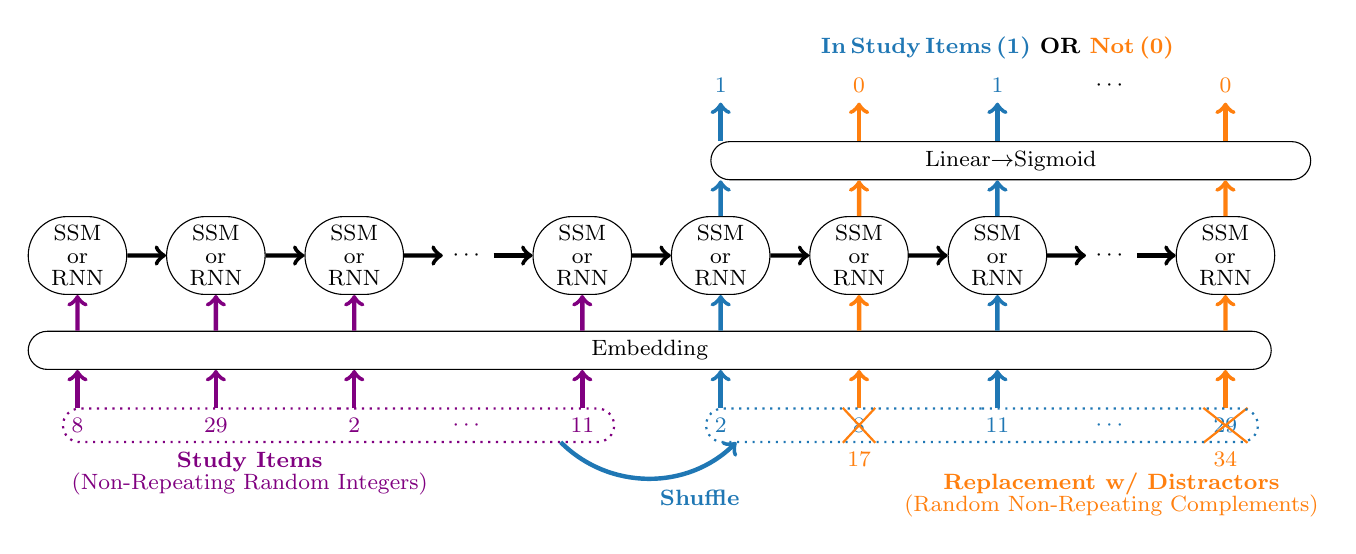
\begin{tikzpicture}[node distance=1.4em,font=\fontsize{8pt}{8pt}\selectfont]
    % RNN
    \node[rounded rectangle,draw,align=center] (RNN1) at (0,0) {SSM\\or\\RNN};
    \node[rounded rectangle,draw,right=of RNN1,align=center] (RNN2) {SSM\\or\\RNN};
    \node[rounded rectangle,draw,right=of RNN2,align=center] (RNN3) {SSM\\or\\RNN};
    \node[right=of RNN3] (RNN_dots) {$\cdots$};
    \node[rounded rectangle,draw,right=of RNN_dots,align=center] (RNN4) {SSM\\or\\RNN};
    \node[rounded rectangle,draw,right=of RNN4,align=center] (RNN5) {SSM\\or\\RNN};
    % \node[right=of RNN5] (RNN_dots2) {$\cdots$};
    \node[rounded rectangle,draw,right=of RNN5,align=center] (RNN6) {SSM\\or\\RNN};
    \node[rounded rectangle,draw,right=of RNN6,align=center] (RNN7) {SSM\\or\\RNN};
    \node[right=of RNN7] (RNN_dots2) {$\cdots$};
    \node[rounded rectangle,draw,right=of RNN_dots2,align=center] (RNN8) {SSM\\or\\RNN};
    \draw[->,ultra thick] (RNN1) -- (RNN2);
    \draw[->,ultra thick] (RNN2) -- (RNN3);
    \draw[->,ultra thick] (RNN3) -- (RNN_dots);
    \draw[->,ultra thick] (RNN_dots) -- (RNN4);
    \draw[->,ultra thick] (RNN4) -- (RNN5);
    \draw[->,ultra thick] (RNN7) -- (RNN_dots2);
    \draw[->,ultra thick] (RNN_dots2) -- (RNN8);
    \draw[->,ultra thick] (RNN6) -- (RNN7);
    \draw[->,ultra thick] (RNN5) -- (RNN6);
    % % Embedding
    % % t=1
    % \node[below=1.5em of RNN1,rectangle,fill=black!6.3822,minimum size=0.025em] (embed1_1) {};
    %     \node[anchor=north,rectangle,fill=black!71.1932,minimum size=0.025em] (embed1_2) at (embed1_1.south) {};
    %     % \node[anchor=north,rectangle,minimum size=0.05em] (embed1_3) at (embed1_2.south) {\scalebox{0.5}{$\mathbb{\vdots}$}};
    %     \node[anchor=north,rectangle,fill=black!28.4883,minimum size=0.05em,yshift=-0.5em] (embed1_4) at (embed1_2.south) {};
    %     \draw[densely dotted,thick] (embed1_2.south) -- (embed1_4.north);
    %     \draw[violet,ultra thick] (embed1_1.north west) rectangle (embed1_4.south east);
    % % t=2
    % \node[below=1.5em of RNN2,rectangle,fill=black!43.4254,minimum size=0.025em] (embed2_1) {};
    %     \node[anchor=north,rectangle,fill=black!28.9347,minimum size=0.025em] (embed2_2) at (embed2_1.south) {};
    %     % \node[anchor=north,rectangle,minimum size=0.05em] (embed2_3) at (embed2_2.south) {\scalebox{0.5}{$\mathbb{\vdots}$}};
    %     \node[anchor=north,rectangle,fill=black!99.3098,minimum size=0.05em,yshift=-0.5em] (embed2_4) at (embed2_2.south) {};
    %     \draw[densely dotted,thick] (embed2_2.south) -- (embed2_4.north);
    %     \draw[violet,ultra thick] (embed2_1.north west) rectangle (embed2_4.south east);
    % % t=3
    % \node[below=1.5em of RNN3,rectangle,fill=black!13.5946,minimum size=0.025em] (embed3_1) {};
    %     \node[anchor=north,rectangle,fill=black!78.9994,minimum size=0.025em] (embed3_2) at (embed3_1.south) {};
    %     % \node[anchor=north,rectangle,minimum size=0.05em] (embed3_3) at (embed3_2.south) {\scalebox{0.5}{$\mathbb{\vdots}$}};
    %     \node[anchor=north,rectangle,fill=black!5.0599,minimum size=0.05em,yshift=-0.5em] (embed3_4) at (embed3_2.south) {};
    %     \draw[densely dotted,thick] (embed3_2.south) -- (embed3_4.north);
    %     \draw[violet,ultra thick] (embed3_1.north west) rectangle (embed3_4.south east);
    % % dots
    % \node[] (embed_dots) at (RNN_dots|-embed1_2.south) {$\cdots$};
    % % t=4
    % \node[below=1.5em of RNN4,rectangle,fill=black!24.0146,minimum size=0.025em] (embed4_1) {};
    %     \node[anchor=north,rectangle,fill=black!44.4282,minimum size=0.025em] (embed4_2) at (embed4_1.south) {};
    %     % \node[anchor=north,rectangle,minimum size=0.05em] (embed4_3) at (embed4_2.south) {\scalebox{0.5}{$\mathbb{\vdots}$}};
    %     \node[anchor=north,rectangle,fill=black!15.9579,minimum size=0.05em,yshift=-0.5em] (embed4_4) at (embed4_2.south) {};
    %     \draw[densely dotted,thick] (embed4_2.south) -- (embed4_4.north);
    %     \draw[violet,ultra thick] (embed4_1.north west) rectangle (embed4_4.south east);
    % % t=5
    % \node[below=1.5em of RNN5,rectangle,fill=black!13.5946,minimum size=0.025em] (embed5_1) {};
    %     \node[anchor=north,rectangle,fill=black!78.9994,minimum size=0.025em] (embed5_2) at (embed5_1.south) {};
    %     % \node[anchor=north,rectangle,minimum size=0.05em] (embed5_3) at (embed5_2.south) {\scalebox{0.5}{$\mathbb{\vdots}$}};
    %     \node[anchor=north,rectangle,fill=black!5.0599,minimum size=0.05em,yshift=-0.5em] (embed5_4) at (embed5_2.south) {};
    %     \draw[densely dotted,thick] (embed5_2.south) -- (embed5_4.north);
    %     \draw[blue,ultra thick] (embed5_1.north west) rectangle (embed5_4.south east);
    % % dots2
    % \node[] (embed_dots2) at (RNN_dots2|-embed1_2.south) {$\cdots$};
    % % t=6
    % \node[below=1.5em of RNN6,rectangle,fill=black!33.8048,minimum size=0.025em] (embed6_1) {};
    %     \node[anchor=north,rectangle,fill=black!17.7876,minimum size=0.025em] (embed6_2) at (embed6_1.south) {};
    %     % \node[anchor=north,rectangle,minimum size=0.05em] (embed6_3) at (embed6_2.south) {\scalebox{0.5}{$\mathbb{\vdots}$}};
    %     \node[anchor=north,rectangle,fill=black!42.1924,minimum size=0.05em,yshift=-0.5em] (embed6_4) at (embed6_2.south) {};
    %     \draw[densely dotted,thick] (embed6_2.south) -- (embed6_4.north);
    %     \draw[orange,ultra thick] (embed6_1.north west) rectangle (embed6_4.south east);
    % % t=7
    % \node[below=1.5em of RNN7,rectangle,fill=black!24.0146,minimum size=0.025em] (embed7_1) {};
    %     \node[anchor=north,rectangle,fill=black!44.4282,minimum size=0.025em] (embed7_2) at (embed7_1.south) {};
    %     % \node[anchor=north,rectangle,minimum size=0.05em] (embed7_3) at (embed7_2.south) {\scalebox{0.5}{$\mathbb{\vdots}$}};
    %     \node[anchor=north,rectangle,fill=black!15.9579,,minimum size=0.05em,yshift=-0.5em] (embed7_4) at (embed7_2.south) {};
    %     \draw[densely dotted,thick] (embed7_2.south) -- (embed7_4.north);
    %     \draw[blue,ultra thick] (embed7_1.north west) rectangle (embed7_4.south east);
    % % t=8
    % \node[below=1.5em of RNN8,rectangle,fill=black!36.3285,minimum size=0.025em] (embed8_1) {};
    %     \node[anchor=north,rectangle,fill=black!60.9385,minimum size=0.025em] (embed8_2) at (embed8_1.south) {};
    %     % \node[anchor=north,rectangle,minimum size=0.05em] (embed8_3) at (embed8_2.south) {\scalebox{0.5}{$\mathbb{\vdots}$}};
    %     \node[anchor=north,rectangle,fill=black!68.8193,minimum size=0.05em,yshift=-0.5em] (embed8_4) at (embed8_2.south) {};
    %     \draw[densely dotted,thick] (embed8_2.south) -- (embed8_4.north);
    %     \draw[orange,ultra thick] (embed8_1.north west) rectangle (embed8_4.south east);
    % \draw[->,ultra thick,violet] (embed1_1) -- (RNN1);
    % \draw[->,ultra thick,violet] (embed2_1) -- (RNN2);
    % \draw[->,ultra thick,violet] (embed3_1) -- (RNN3);
    % \draw[->,ultra thick,violet] (embed4_1) -- (RNN4);
    % \draw[->,ultra thick,blue] (embed5_1) -- (RNN5);
    % \draw[->,ultra thick,orange] (embed6_1) -- (RNN6);
    % \draw[->,ultra thick,blue] (embed7_1) -- (RNN7);
    % \draw[->,ultra thick,orange] (embed8_1) -- (RNN8);
    % Embedding layer
    \path let \p1=(RNN1.west), \p2=(RNN8.east) in (RNN1) to (RNN8)
        node[anchor=west, minimum width=\x2-\x1+0.5em, rounded rectangle, draw,yshift=-2em] (embed_layer)
        at (RNN1.west|-RNN8.south)%embed8_4.south)
        {Embedding};
    \draw[->,ultra thick,violet] (RNN1|-embed_layer.north) -- (RNN1);%(embed1_4);
    \draw[->,ultra thick,violet] (RNN2|-embed_layer.north) -- (RNN2);%(embed2_4);
    \draw[->,ultra thick,violet] (RNN3|-embed_layer.north) -- (RNN3);%(embed3_4);
    \draw[->,ultra thick,violet] (RNN4|-embed_layer.north) -- (RNN4);%(embed4_4);
    \draw[->,ultra thick,blue] (RNN5|-embed_layer.north) -- (RNN5);%(embed5_4);
    \draw[->,ultra thick,orange] (RNN6|-embed_layer.north) -- (RNN6);%(embed6_4);
    \draw[->,ultra thick,blue] (RNN7|-embed_layer.north) -- (RNN7);%(embed7_4);
    \draw[->,ultra thick,orange] (RNN8|-embed_layer.north) -- (RNN8);%(embed8_4);
    % inputs
    \node[yshift=-2em,text=violet] (input1) at (RNN1|-embed_layer.south) {8};
    \node[text=violet] (input2) at (RNN2|-input1) {29};
    \node[text=violet] (input3) at (RNN3|-input1) {2};
    \node[text=violet] (input_dots) at (RNN_dots|-input1) {$\cdots$};
    \node[text=violet] (input4) at (RNN4|-input1) {11};
    \node[text=blue] (input5) at (RNN5|-input1) {2};
    \node[text=blue] (input_dots2) at (RNN_dots2|-input1) {$\cdots$};
    \node[text=blue,shape=cross out,draw=orange,thick] (input6) at (RNN6|-input1) {8};
    \node[text=orange,anchor=north] (input6other) at (input6.south) {17};
    \node[text=blue] (input7) at (RNN7|-input1) {11};
    \node[text=blue,shape=cross out,draw=orange,thick] (input8) at (RNN8|-input1) {29};
    \node[text=orange,anchor=north] (input8other) at (input8.south) {34};
    \draw[->,ultra thick,violet] (input1) -- (RNN1|-embed_layer.south);
    \draw[->,ultra thick,violet] (input2) -- (RNN2|-embed_layer.south);
    \draw[->,ultra thick,violet] (input3) -- (RNN3|-embed_layer.south);
    \draw[->,ultra thick,violet] (input4) -- (RNN4|-embed_layer.south);
    \draw[->,ultra thick,blue] (input5) -- (RNN5|-embed_layer.south);
    \draw[->,ultra thick,orange] (input6) -- (RNN6|-embed_layer.south);
    \draw[->,ultra thick,blue] (input7) -- (RNN7|-embed_layer.south);
    \draw[->,ultra thick,orange] (input8) -- (RNN8|-embed_layer.south);
    \node[anchor=north west,align=center,text=violet] (input_ann) at (input1.south west) {\textbf{Study Items}\\(Non-Repeating Random Integers)};
    % Filler
    \node[anchor=north,align=center,text=orange,yshift=0.5em] (other) at (input6other.south-|input_dots2) {\textbf{Replacement w/ Distractors}\\(Random Non-Repeating Complements)};
    % Reaout layer
    \path let \p1=(RNN5.west), \p2=(RNN8.east) in (RNN5) to (RNN8)
        node[above=2em of RNN5.north west, anchor=west, minimum width=\x2-\x1+0.5em, rounded rectangle, draw] (readout_layer) {Linear$\to$Sigmoid};
    \draw[->,ultra thick,blue] (RNN5) -- (RNN5|-readout_layer.south);
    \draw[->,ultra thick,orange] (RNN6) -- (RNN6|-readout_layer.south);
    \draw[->,ultra thick,blue] (RNN7) -- (RNN7|-readout_layer.south);
    \draw[->,ultra thick,orange] (RNN8) -- (RNN8|-readout_layer.south);
    % output for palindrome
    \node[text=blue,yshift=2em] (sort5) at (RNN5|-readout_layer.north) {1};
    \node (sort_dots) at (RNN_dots2|-sort5) {$\cdots$};
    \node[text=orange] (sort6) at (RNN6|-sort5) {0};
    \node[text=blue] (sort7) at (RNN7|-sort5) {1};
    \node[text=orange] (sort8) at (RNN8|-sort5) {0};
    \draw[->,ultra thick,blue] (RNN5|-readout_layer.north) -- (sort5);
    \draw[->,ultra thick,orange] (RNN6|-readout_layer.north) -- (sort6);
    \draw[->,ultra thick,blue] (RNN7|-readout_layer.north) -- (sort7);
    \draw[->,ultra thick,orange] (RNN8|-readout_layer.north) -- (sort8);
    \node[anchor=south] (sort_ann) at (sort7.north) {\textbf{{\color{blue}{In\,Study\,Items\,(1)}} OR \color{orange}{Not\,(0)}}};
    \path let \p1=(input1.west), \p2=(input4.east) in (input1) to (input4)
        node[anchor=west, minimum width=\x2-\x1+1em, rounded rectangle, draw, dotted,thick,violet] (inputs) at (input1.west|-input4.east) {\phantom{M}};
    \path let \p1=(input5.west), \p2=(input8.east) in (input5) to (input8)
        node[anchor=west, minimum width=\x2-\x1+1em, rounded rectangle, draw, dotted,thick,blue] (shuffled) at (input5.west|-input8.east) {\phantom{M}};
    % \draw [decoration={brace,mirror,amplitude=0.5em},decorate,ultra thick,violet] (input1.south west) -- (input4.south east);
    % \draw [decoration={brace,mirror,amplitude=0.5em},decorate,ultra thick,violet] (input5.south west) -- (input8.south east);
    \draw[->,ultra thick,blue] (input4.south west) to [bend right=45] node [below,anchor=north west] {\textbf{Shuffle}} (input5.south east);
    \end{tikzpicture}
	\caption{Schematic illustration of the binary memory verification task.}
	\label{fig:task}
\end{figure*}

Since the Transformer architecture is inherently position-agnostic---lacking an intrinsic ordering mechanism apart from external positional encodings \citep{Vaswani+17_AttentionIsAllYouNeed}---the primacy effects observed in these studies must stem from the statistical properties of the training data or task design.
\citeauthor{Wang+23_primacy-effect} argued that LLMs inherit cognitive biases from human-generated linguistic data.
\citeauthor{Xiao+24} suggested that the nature of the language modeling task itself encourages prioritization of initial tokens, as they are repeatedly used as inputs for autoregressive predictions, reinforcing attention allocation to them.



In contrast to prior investigations, the present study examines the emergence of the primacy effect in ANNs preventing the inheritance of human-induced bias.
Specifically, the models are trained on a synthetic memorization task designed based on psychological experiments conducted with humans and other animals \citep{ThompsonHerman77,SandsWright80,Wright+85}.
The following section details the task formulation and the model architecture.



\section{Methods}

\subsection{Task}

The memorization patterns of ANNs were assessed using the binary memory verification task \citep[Fig.~\ref{fig:task}; a.k.a. \emph{serial probe recognition};][]{WickelgrenNorman66,ThompsonHerman77,SandsWright80,Wright+85}.%
\footnote{
	The most widely adopted task for assessing the primacy effect in human memory is \emph{free recall}, in which participants are presented with a sequence of items and subsequently asked to recall them in an order-agnostic manner \citep{Murdock62,GlanzerCunitz66}. 
	While this paradigm can be technically formulated as a loss function for ANNs \citep{Cuturi13}, initial explorations of this study revealed that model performance remained suboptimal under this approach, yielding lower accuracy than in theoretically more demanding tasks requiring order-sensitive reconstruction.
	Consequently, the present study adopted the more machine learning-friendly task based on binary verification.
	Remarkably, this task has also been used to assess the memory capacity of non-human animals, which are unable to perform free recall \citep{ThompsonHerman77,SandsWright80,Wright+85}.
}
In this task, the models were first presented with a sequence of randomly generated, non-repeating integers (hereinafter referred to as \emph{study items}).
Subsequently, they received another sequence of integer queries and were trained to determine whether each query token was present (labeled as 1) or absent (labeled as 0) in the study items.
To construct these queries, the study items were first shuffled, and then, with a probability of $p=0.5$, each shuffled token was replaced with a randomly sampled integer from the complement set of the study items (termed \emph{distractors}).


The task hyperparameters were manually adjusted to prevent the models from achieving perfect accuracy.
Specifically, the input length was set to $L \in \{64, 128, 256\}$, and the vocabulary size was fixed at $K:=4096$.
% 
Each model underwent ten independent training runs with different random seeds.
For evaluation, 1024 sets of integers were held out as test data, ensuring that these integer combinations never appeared as study items in the training set, regardless of their order.

To build test sequences, the held-out study items were randomly ordered, and queries were generated by first shuffling and then cyclically shifting them (e.g., $(2,8,11,29) \mapsto \{ (2,8,11,29), (8,11,29,2), (11,29,2,8), (29,2,8,11) \}$).
This design ensured that each study item was queried in all $L$ possible positions.
Finally, either the even- or odd-indexed query positions were replaced with random distractors, resulting in a total of $1024 \times L \times 2$ test sequences per trial.


\subsection{Models}

The models used for the binary memory verification task comprised three layers, as illustrated in Fig.~\ref{fig:task}.
In the first layer, the input integers were embedded into 256-dimensional real-valued vectors.
These embeddings were shared between study items and query tokens.
The resulting sequence of vectors was then processed by the SSM/RNN, whose outputs were linearly projected onto binary logits to determine whether each query token was present in the study items.

This study primarily examined the single-layer S4 model as the goldstandard implementation of the SSM \citep{Gu+22}.%
\footnote{
	Recent studies have shown that the state matrix ($A$) of S4 can be simplified into a purely diagonal form without compromising performance \citep[S4D;][]{Gu+22_S4D}.
	By contrast, the original S4 model introduced an additional low-rank component to the diagonal structure (referred to as the Diagonal Plus Low Rank form, or DPLR) to ensure a mathematically well-founded state matrix.
	Notably, the diagonal variant exhibited a qualitatively similar primacy effect to the DPLR model.
	Due to the page limitations, results for the diagonal model are omitted from this paper, and all reported findings are based on the DPLR model.}
The model encoded the channel-wise dynamics of the input embeddings in a complex-valued space, with its outputs subsequently projected back into the real domain by discarding imaginary components.
The state and input matrices ($A$ and $B$ in Eq.~\ref{eq:ssm}) were initialized to approximate each channel's trajectory using Legendre/Laguerre polynomials of degrees 0--63 (HiPPO-LegS/LagT)
or a Fourier basis $\{ s_0,c_0,\dots,s_{31},c_{31} \}$, where $s_n(t) := \sqrt{2}\sin(2\pi n t)$ and $c_n(t) := \sqrt{2}\cos(2\pi n t)$ \citep[HiPPO-Fout, Fourier Recurrent Unit;][]{Zhang+18_FRU,Gu+20,Gu+23_ICLR}.
The matrices were discretized by the bilinear method \citep{Tustin47}.
% The dimensionality of the state space per channel (i.e., the degree of the polynomials approximating each channel's trajectory) was set as 64.

For comparison, a single-layer long short-term memory (LSTM) network was also evaluated \citep[][]{HochreiterSchmidhuber97_LSTM}.
LSTM
% Two RNNs were also tested as baselines.
% One of them was the long short-term memory \citep[LSTM;][]{HochreiterSchmidhuber97_LSTM}, which 
has been the goldstandard RNN architecture for various time-series processing tasks, including language modeling \citep{Sundermeyer+12,Graves13}.
% The other model was the gated recurrent unit \citep[GRU;][]{Cho+14_GRU}, which simplied the LSTM and achieved faster computation suitable for waveform modeling etc. \citep{Kalchbrenner+18}.
% Both LSTM and GRU were single-layered and the dimensionality of their hidden state was 256.
% The LSTM was also equipped with another module for memory storage (called the cell state) of the same dimensionality of 256.
The dimensionality of both hidden and cell states was set to 256.

Another well-established baseline worth considering is the Transformer architecture \citep[][]{Vaswani+17_AttentionIsAllYouNeed}, equipped with a sufficiently long memory window.
However, it turned out that the Transformer can easily achieve perfect accuracy on the adopted task---even at the maximal levels of input length and vocabulary size implementable within the available computational resources---thereby failing to incur the memory load necessary for evaluating the primacy effect%
\footnote{
	For the same reason, the proposed experimental paradigm was also inadequate for testing extended architectures of the SSM \citep[Mamba;][]{GuDao24,DaoGu24} and the LSTM \citep[xLSTM;][]{Beck+24}, both of which attained perfect accuracy at the highest task difficulty settings.}
Consequently, the Transformer is excluded from the main results reported in the next section; instead, the Appendix provides a detailed explanation of how it can solve the memory verification task, with particular emphasis on the role of its attention mechanism.

The models were trained for 300,000 iterations using the Adam optimizer with parameters $(\beta_0,\beta_1) := (0.9,0.99)$ \citep{KingmaBa15_Adam}.
Batch size was set to 512.
The learning rate was linearly increased from 0.0 to 0.001 over the first 1,000 iterations (\emph{warmups}) and subsequently decayed according to the cosine annealing schedule \cite{LoshchilovHutter17}.
To prevent gradient explosion, the gradient norm was clipped at 1.0.
The Python code for the experiments is available at \url{https://github.com/An0nym0usAuth0r/NeuralPrimacyEffect.git}.



\section{Results}

\subsection{Emergence of the Primacy Effect}

Fig.~\ref{fig:accuracy} reports the accuracy of the binary memory verification task across all combinations of memorization and verification times.
The brightness of each cell in the square heatmaps indicates the accuracy for study items that were presented at the time indexed by the corresponding row and queried at the time indexed by the corresponding column.
That is, they report the proportion of true positives against false negatives (i.e., the \emph{recall} score).
Additionally, the top separate row of each panel displays the accuracy for distractor queries (integers not included among the study items), capturing the prevalence of true negatives over false positives.
Just below it, the second row summarizes the average accuracy across memorization times (rows).
Similarly, the rightmost separate column represents the average accuracy across all verification times (columns).

The binary memory verification performance of the SSM model was highest for study items presented at the beginning of the sequence, demonstrating a clear primacy effect (Fig.~\ref{fig:trained_nplr}--\subref{fig:frozen_long}).
The model maintained high accuracy across different query timings (as indicated by the bright colors in the top rows of the heatmaps), provided that the sequence length did not exceed its capacity (see the accuracy decline in Fig.~\ref{fig:frozen_long}, where $L=256$).
In other words, memory for the initial study items exhibited minimal decay over time.
% This attested pattern demonstrates the primacy effect in the SSM.

By contrast, the LSTM did not display this primacy effect; its accuracy was uniform across both the memorization and verification phases (Fig.~\ref{fig:lstm}).

Interestingly, the SSM's accuracy for the most recently presented study items was lowest when they were queried immediately after their initial presentation in the memorization phase (indicated by the dark colors in the bottom-left region of the heatmaps).
This suggests a temporal delay between the encoding of study items and their effective retrieval.
% To put it differently, there was a delay after the study items were presented and before the model became able to retrieve them.
% This attested pattern characterizes 

These findings held true regardless of whether the state and input matrices of the SSM were optimized for the task (Fig.~\ref{fig:trained_nplr}) or remained fixed at their initial values (Fig.~\ref{fig:frozen_nplr}--\subref{fig:frozen_long}).
Moreover, the results remained consistent across different polynomial bases underlying the state and input matrices, including Laguerre (Fig.~\ref{fig:frozen_lagt}), Fourier (\ref{fig:frozen_fout}), and Legendre (all other panels).

% the key parameter, $\Delta t$ (discretization time-step size), can be represented near-linearly (Fig.~\ref{fig:frozen_softplus}) or in log scale (Fig.~\ref{fig:trained_nplr}, \subref{fig:frozen_nplr}, \subref{fig:frozen_dt-1.0}--\subref{fig:frozen_long}), and its initial values can be distributed over a wider range ($0.001 \leq \Delta t \leq 1.0$; Fig.~\ref{fig:frozen_dt-1.0}) than the standard ($0.001 \leq \Delta t \leq 0.1$; Fig.~\ref{fig:trained_nplr}--\subref{fig:frozen_softplus}, \subref{fig:frozen_short}, \subref{fig:frozen_long}).

\begin{figure*}
	\begin{subcaptiongroup}
		\phantomcaption\label{fig:trained_nplr}
		% \phantomcaption\label{fig:trained_diag}
		\phantomcaption\label{fig:frozen_nplr}
		\phantomcaption\label{fig:frozen_lagt}
		\phantomcaption\label{fig:frozen_fout}
		% \phantomcaption\label{fig:frozen_diag}
		% \phantomcaption\label{fig:frozen_softplus}
		\phantomcaption\label{fig:frozen_dt-1.0}
		\phantomcaption\label{fig:frozen_short}
		\phantomcaption\label{fig:frozen_long}
		% \phantomcaption\label{fig:gru}
		\phantomcaption\label{fig:lstm}
	\end{subcaptiongroup}
	\centering
	\includegraphics[width=0.9\linewidth]{figs/verification.pdf}
	\caption{Accuracy of the binary memory verification task.
	Each cell in the square heatmaps represents the accuracy (or the recall score) for study items that were presented at the time indexed by the corresponding row and queried at the time indexed by the corresponding column. The accuracy for distractor queries is displayed in the top separate row of each panel, alongside the average accuracy across memorization times (rows). Similarly, the rightmost separate column represents the average accuracy across verification times (columns).
	% rows correspond to the input time indices of the test study items, and the columns to those of the queries.
	The bottom-right panel (\subref{fig:lstm}) depicts the accuracy distribution for the LSTM, while the other panels (\subref{fig:trained_nplr}--\subref{fig:frozen_long}) report results for the SSM (S4) model under different parameter configurations.
	The state and input matrices of the SSM were initialized to approximate the latent dynamics of input sequences using Legendre polynomials, except in panels \subref{fig:frozen_lagt} and \subref{fig:frozen_fout}, where Laguerre and Fourier bases were used, respectively.
	The state and input matrices were optimized for the task in panel \subref{fig:trained_nplr}, whereas they remained fixed at their initial values in all other panels.
	% the state matrix $A$ was ``Diagonal'' (B,D) or DPLR (otherwise);
	The discretization step size $\Delta t$ was 
	% parameterized in the $\mathrm{Softplus}^{-1}$ space (\subref{fig:frozen_softplus}) or log space (\subref{fig:trained_nplr}, \subref{fig:frozen_nplr}, \subref{fig:frozen_dt-1.0}--\subref{fig:frozen_long}), and 
	initialized in the range $0.001 \leq \Delta t \leq 0.1$, except in panel \subref{fig:frozen_dt-1.0}, where the upper bound was extended to $1.0$ (i.e., $0.001 \leq \Delta t \leq 1.0$).
	% (\subref{fig:trained_nplr}--\subref{fig:frozen_softplus}, \subref{fig:frozen_short}, \subref{fig:frozen_long}).
	% The bottom two panels report the results of two goldstandard RNNs, GRU (\subref{fig:gru}) and LSTM (\subref{fig:lstm}) for comparison.
	The number of study items was set to $L=128$, except in panel \subref{fig:frozen_short} ($L=64$) and panel \subref{fig:frozen_long} ($L=256$).
	}
	\label{fig:accuracy}
\end{figure*}

\begin{figure*}
	\centering
	\includegraphics[width=1.0\linewidth]{figs/verification_dt.pdf}
	\caption{Top row: Optimization trajectories of the discretization step size $\Delta t$ in the SSM (S4) model with frozen Legendre state and input matrices. Each heatmap column represents the distribution of $\Delta t$ across 256 latent channels $\times$ 10 training runs, sorted in the ascending order.
	Bottom row: Histograms displaying the initial (blue) and final (orange) values of $\Delta t$, aggregated across the 256 latent channels $\times$ 10 training runs (see Fig.~\ref{fig:delta-t_per-seed} in the Appendix for variations among individual runs).
	The first to third panel columns from the left show the results for three different ranges of log-uniformly random initializations, whereas the fourth and fifth columns tested shorter and longer study items, respectively.
	}
	\label{fig:delta-t}
\end{figure*}


\subsection{Distribution of the Time-Step Sizes}

As discussed in the Preliminaries, the discretization time-step size $\Delta t$ plays a critical role in determining the memory capacity of the SSM.
Moreover, once the state matrix $A$ is fixed, $\Delta t$ becomes the sole parameter capable of influencing the \emph{dynamics} of the SSM;%
\footnote{
	Freezing $\Delta t$ resulted in a complete failure of learning.}
all remaining parameters are confined to \emph{feedforward} transforms.
% although the primacy effect emerged across different initial values (Fig.~\ref{fig:frozen_dt-1.0}).

Accordingly, to further investigate its role, the optimization trajectories of $\Delta t$ were tracked over the course of training.
The analysis revealed that as training progressed, a specific range of step sizes ($\Delta t \leq 0.03$) became dominant, compensating for the deallocation of the higher range approximately between 0.03 and 0.2 (Fig.~\ref{fig:delta-t}).

Additionally, the peak value of $\Delta t$ was found to depend on the number of the study items $L$; longer study sequences led the model to favor smaller $\Delta t$ values (compare the leftmost panel with the two rightmost panels).



\section{Discussions}

\subsection{Summary of the Findings}

The present study demonstrated that the SSM exhibits the primacy effect in memorization.
When performing the binary memory verification task, which parallels paradigms used to investigate memory capacity in humans and animals \citep{WickelgrenNorman66,ThompsonHerman77,SandsWright80,Wright+85}, the model showed the highest accuracy for study items presented at the beginning of the sequence.
Moreover, memorized information was not retrievable immediately after the presentation of the study items.
These findings are novel and counterintuitive, as they challenge the theoretical formulation of the SSM, which assumes an exponentially decaying measure \citep[for Legendre and Laguerre bases; Fig~\ref{fig:kernel};][]{Gu+23_ICLR}.


As noted in the Preliminaries, the SSM was designed to achieve a longer-lasting memory than classical RNNs \citep{Gu+20}.
Prior research on RNNs and SSMs has focused on their ability to preserve input data against temporal decay.
A typical benchmark for these inquiries is the delayed reconstruction task \citep[a.k.a. the \emph{copying memory task};][]{Arjovsky+16}.
In this task, models are provided with a \emph{short} sequence of integers---usually ten repeatable random samples ranging between 0 and 7---followed by null inputs (e.g., zero vectors), and are then asked to reconstruct the initially observed sequence in the original order.
Model performance is evaluated based on the length of the null-valued interval between the initial observations and their reconstructions.


However, little attention has been given to how the model handles longer study sequences and larger vocabularies when memory capacity reaches its limit.%
\footnote{
	It should be noted that the performance of the SSM can be enhanced by increasing the number of layers and/or latent channels.
	In this study, the model's capacity was intentionally constrained in order to study its behavior under conditions where perfect accuracy is unattainable.
}
In particular, the question of whether the models prioritize initial/middle/recent observations has remained unexplored.
The present study addressed this question and discovered that the SSM predominantly preserved the initial observations.

The key factor responsible for the primacy effect in the SSM appears to be the time-step size, $\Delta t$, as all the other trainable parameters pertain exclusively to feedforward transforms.
After training on the memorization task, $\Delta t$ values concentrated below a specific threshold ($\Delta t \leq 0.03$).
As discussed in the Preliminaries, smaller $\Delta t$ values allow the model to retain more distant memories, while larger $\Delta t$ values enhance the discrimination of adjacent tokens \citep[][]{Gu+21,GuDao24}.
The learning results thus align with the \emph{necessary} condition for the primacy effect;
however, the question remains as to why recent observations were remembered less accurately despite the exponentially decaying measure underlying the polynomial-approximation theory.

The SSMs analyzed in this study were trained from scratch on a synthetic memorization task that was designed to closely resemble controlled psychological experiments \citep{WickelgrenNorman66,ThompsonHerman77,SandsWright80,Wright+85}.
Consequently, the observed primacy effect is attributed to the intrinsic properties of the SSM per se, rather than to biases introduced by data or task design.
From this perspective, the the present study stands in contrast to prior investigations of LLMs \citep{Wang+23_primacy-effect,EicherIrgolic24,GuoVosoughi24,Janik24,Liu+24,Xiao+24};
LLMs are trained on human-generated linguistic data and therefore likely to inherit the primacy effect as a byproduct of human cognitive biases embedded in the data.

\subsection{Implications for Computational Neuroscience}

Most existing theories of the primacy effect in human and animal memory have focused on abstract, procedural explanations of the cognitive bias.
One influential account is the dual-store hypothesis \citep[][]{WaughNorman65,GlanzerCunitz66,AtkinsonShiffrin68}, which attributes the primacy and recency effects to two distinct memory systems.
According to this view,study items presented early in a sequence are transferred from short-term memory---where all incoming observations are temporally buffered---into long-term memory, where they are preserved against decay, thereby producing the primacy effect.
By contrast, the recency effect is thought to arise from the residual information retained in short-term memory, which has limited capacity and only holds the most recent inputs.
% \citet{Neath93} and \citet{NeathKnoedler94} introduced the distinctiveness score of study items based on the ellapsed time from their presentation to the recall and the relative differences of these values among the items.

Moving beyond such abstract accounts, several researchers have proposed biologically grounded neural network models that replicate the primacy effect \citep{Burgess+91,Wong+91,Greene+00,Sikstrom06,Lansner+13}.
The present findings align with this line of work but offer a novel perspective.
Specifically, the SSM examined here was developed with the aim of advancing practically useful artificial intelligence, independently of any deliberate attempt to model the primacy effect from a psychological/biological standpoint.
Thus, the spontaneous emergence of the primacy effect in the SSM presents a unique and complementary hypothesis for the mechanism underlying this cognitive bias, opening new avenues for future investigation in computational neuroscience.
% while the existing models had 
% may contribute to the development of a novel and more neurobiologically grounded model of the primacy effect.


Importantly, the industrial orientation of the SSM does not imply biological implausibility.
\citet{VoelkerEliasmith18} and \citet{Voelker+19} established a connection between the SSM and spiking neural networks, demonstrating that the dynamics of the state vector in the SSM (Eq.~\ref{eq:ssm}) can be implemented using a population of spiking neurons, which remain the most plausible model of biological neuronal activity to date.
% , a spiking version of the SSM studied here could serve as a new neurobiological model of the primacy effect.
Moreover, \citet{VoelkerEliasmith18} showed that the spiking instantiation of the SSM, when tuned to implement some particular function known as the \emph{delay line}, reproduces the characteristic behavior of biological \emph{time cells},%
\footnote{
	Time cells fire at specific moments following onset cues/events and are believed to encode temporal information \citep{MacDonald+11}.
}
which have been observed in several brain regions, including the hippocampus \citep{MacDonald+11,Eichenbaum14}, striatum \citep{Mello+15}, and cortex \citep{Luczak+15}.
Comparing a spiking implementation of the SSM exhibiting the primacy effect with brain recordings from psychological experiments may thus yield novel insights into the neuro-computational mechanisms underlying this cognitive phenomenon.
% \citep{MacDonald+11,Eichenbaum14,Mello+15,Luczak+15,Tiganj+16}.

Of course, the present study has certain limitations as a biological simulation.
Most notably, the model here was explicitly optimized for the memorization task from scratch, whereas the primacy effect observed in humans and animals is presumably an outcome of their natural cognitive development.
Thus, fundamentally different mechanisms may underlie the similar memorization biases exhibited by the SSM and biological organisms.
Future studies may address this discrepancy by training the model in a more biologically naturalistic setting.
However, as discussed in the previous section, training an ANN on empirical data, such as natural language, introduces the risk of conflating human-originated cognitive biases---transferred through the data---with the model's intrinsic properties.



It is also important to note that the SSM does not constitute a comprehensive model of sequence memorization;
its lack of the recency effect suggests the necessity of incorporating an additional module to account for short-term memory processes.
% \footnote{
% 	A simple candidate for modeling short-term memory is a finite-queue/Markov system, whose explicitly bounded memory length provides a direct computational account of the well-known ``magic number $7 \pm 2$'' \citep{Miller56}.}
Accordingly, future work should investigate whether the SSM can reliably function as a long-term memory component when integrated with a complementary short-term memory mechanism (e.g., finite-queue/Markov systems), either through modular combination or ensemble learning.


The model's capacity also far exceeded that of biological memory systems.
The binary memory verification task employed in this study involved extremely long lists of study items ($L \in \{64, 128, 256\}$) as well as a huge vocabulary ($K=4096$), which is unlikely to be replicated in human or animal experiments.
This level of task difficulty was necessary to clearly demonstrate the primacy effect in the SSM, and was still insufficient to reach the memory limits of more powerful architectures such as Mamba \citep{GuDao24,DaoGu24} and xLSTM \citep{Beck+24},%
% \footnote{
% 	Mamba and xLSTM attained perfect accuracy even when the input length and vocabulary size were maximally increased within the computational constraints of the present study.}
thereby constraining the scope of model comparison here.
Future research should explore downscaling the model toward more biologically plausible conditions.


Finally, the present study does not offer an explanation for various well-documented characteristics of the psychological primacy effect.
For instance, the retention of initial study items is thought to be achieved, or at least facilitated, by \emph{rehearsal}---repetitive mental or verbal recitation of observed items before requested recall/verification \citep[][%
% see also {\color{red}{more citations}} 
% hockey hamilton 1977
% wixted mcdowell 1977
% wright et al 1990
% castro larsen
% harper mclean dalrymple-alford
% \citealp{Wright+85,Neath93} for its counterevidence
]{Rundus71,MarshallWerder72,Glenberg+80}---for which the models studied here lack an analogous mechanism.

% {\color{red}{Discuss other paradigms/stimuli. e.g. free-recall and image.}}

In addition, the models operated on a unitless discrete time scale, to which the continuous-time representation of the SSM was aligned.
As a result, they are unsuitable for investigating physical-time effects, such as the impact of retention intervals between study-item presentation and verification \citep[][]{CornellBergstrom83,Wright+85,Neath93} or variations in inter-item intervals \citep{NeathKnoedler94}.
% Future studies may address this latter issue by employing more biologically realistic neural network models;
This limitation could be addressed by exploring spiking neural networks equivalent the SSM.
As noted above, the SSM can be converted into a spiking neural network, which in turn enables the simulation of the physical-time effects as well as the incorporation of biologically inspired connectivity structures
\citep{VoelkerEliasmith18}.
% {\color{red}{
% - real-time, interval %\citep{}
% - rehearsal \citep{Rundus71,MarshallWerder72,Glenberg+80}
% }}


% \subsection{Limitations and Future Directions}

% {\color{red}{
% First of all, it should be of note that 
% - model can be enhanced by more layers
% - learning from scratch
% - too much memory capacity
% time cell
% }}

\section*{Acknowledgments}
This study was supported by 
JST ACT-X (JPMJAX21AN) and Core Research for Evolutional Science and Technology (JPMJCR22P5);
JSPS Grant-in-Aid for Early-Career Scientists (JP21K17805) 
and for Scientific Research
A (JP24H00774),
B (JP22H03914),
and C (JP24K15087);
and Kayamori Foundation of Informational Science Advancement (K35XXVIII620).
The author also gratefully acknowledges the support of the
ACCMS, Kyoto University,
regarding the use of their supercomputer system.


\newpage

\bibliographystyle{apalike}

%\setlength{\bibleftmargin}{.125in}
%\setlength{\bibindent}{-\bibleftmargin}

% \bibliography{ccn_style}
\bibliography{takashi_references}

\appendix
% \renewcommand{\thesection}{{Appendix~\Alph{section}}}
% \renewcommand{\section}[1]{\Large\bf \hspace{-0.8em}Appendix: #1}

\section{Appendix}

\begin{figure*}
	\centering
	\includegraphics[width=1.0\linewidth]{figs/verification_dt_per-seed.pdf}
	\caption{Histograms displaying the initial (blue) and final (orange) values of $\Delta t$. Each panel presents the distributions obtained from one of the ten training runs with different random seeds.}
	\label{fig:delta-t_per-seed}
\end{figure*}

\subsection{Remarks on Transformer}
\label{sec:transformer}

As noted in the Methods section, the present study was unable to assess whether or not Transformer exhibits the primacy effect (without inheriting human-induced biases).
Specifically, the model consistently achieved perfect accuracy on the binary memory verification task, thereby failing to encounter the memory load necessary for evaluating the primacy effect.
This section offers a theoretical account of how Transformer is able to solve this task, with particular focus on the role of its attention mechanism.


to begin, recall that the ``memory'' in Transformer (and other finite-queue/Markov models in general) consists of the \emph{raw} input observation, preserved without decay or lossy compression.
Although this approach is highly non-economic for processing long sequences, growing computational resources have made it viable in practice.

Given full access to the uncompressed sequence of prior observations, Transformer computes attention weights based on the dot-product similarity between (linear projected) input embeddings.
In the context of the memory verification task, this computation enables a direct comparison between the study items and verification queries;
setting aside the interference from positional encodings, the resulting attention distribution at each verification time step becomes sharply peaked (one-hot-like) when the query matches a study item, or almost uniform when it does not.
As a result, Transformer can trivially solve the task by exploiting this attention distribution.
% \footnote{
% 	More specifically, suppose that the input-to-value projection is the identity mapping.
% 	Then, when a query matches a study item, the residual connection of this study-item value and the pre-projection query input 
% 	would double (or maximize) the norm  after the residual connection; by contrast, when the query is a previously unobserved distractor, the uniform average of all study-item values would be added to the }

\subsection{Distributions of $\Delta t$ across Training Runs}
\label{sec:delta-t_acorss_runs}


Fig.~\ref{fig:delta-t_per-seed} reports the distribution of the $\Delta t$ parameters before and after each of the ten training runs (decomposing the leftmost panel in Fig.~\ref{fig:delta-t}).


% \lipsum[1-2]

\end{document}
